%versi 2 (8-10-2016) 
\chapter{Pendahuluan}
\label{chap:intro}

\section{Latar Belakang}
\label{sec:label}

Masyarakat kota memerlukan kebutuhan tempat tinggal untuk keberlansungan hidup agar dapat beraktivitas. Agar dapat memenuhi kebutuhan tempat tinggal bagi masyarakat maka pembangunan dan perkembangan pada suatu wilayah harusnya memiliki fungsi lain sebagai Ruang Terbuka Hijau(RTH). RTH merupakan sebuah area yang memanjang atau jalur dan/atau mengelompok,dan penggunaannya yang lebih bersifat terbuka, tempat tumbuh tanaman, baik yang tumbuh secara alamiah maupun yang sengaja ditanam. RTH merupakan penyumbang oksigen terbesar bagi kota. Tentu saja seharusnya RTH tersedia dalam jumlah yang cukup, terutama pada kota yang memiliki penduduk yang banyak.

\begin{figure}[h]
	\centering
	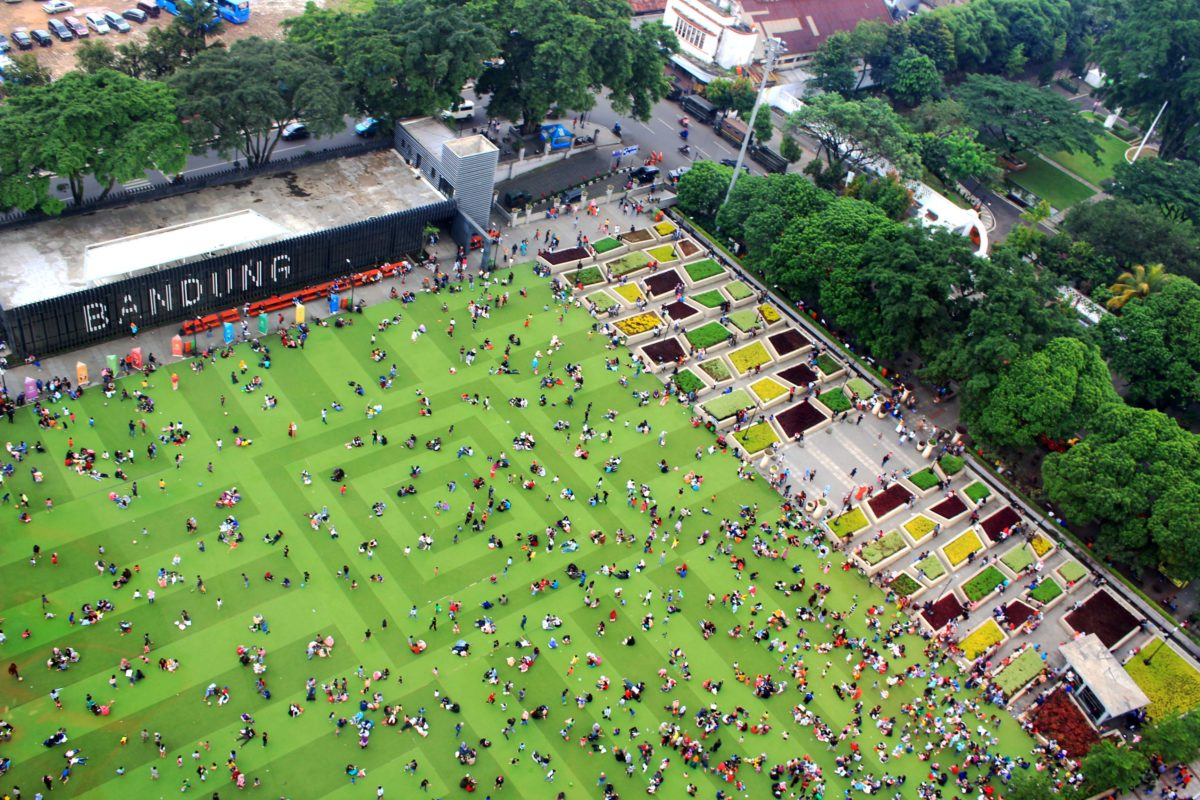
\includegraphics[width=0.7\textwidth]{ruang terbuka hijau.jpg}
	\caption[RTH]{Contoh Ruang Terbuka Hijau\footnote{Ilustrasi ruang terbuka hijau\url{https://www.rth.bandung.go.id/}}}
	
\end{figure}


Pemanfaatan citra satelit merupakan sebuah cara agar dapat mengetahui luas RTH pada suatu kota. Citra Satelit adalah gambaran dari permukaan bumi yang didapatkan langsung dari satelit. Oleh karena itu, citra satelit dapat digunakan dalam mengidentifikasi RTH yang mana terdapatnya banyak pepohonan pada suatu wilayah. Perhitungan juga dapat dilakukan pada citra satelit ,dan hasil dari perhitungan luas RTH pada suatu wilayah diharapkan dapat memberikan dorongan untuk peningkatan dalam penghijauan agar dapat digunakan oleh pemerintah dalam merancang dan meningkatkan penghijauan di berbagai wilayah di Indonesia.


Penelitian yang telah dilakukan \VSM, Fritz H. Silalahi SKom, dan Juan A. Kusjadi menghasilkan data area hijau dari citra satelit pada Kota Bandung yang dibagi menjadi beberapa kelurahan atau kecamatan Kota Bandung. Hasil dari penelitian terdiri dari area hijau untuk 149 kelurahan di 30 kecamatan kota Bandung dan telah selesai dilakukan perhitungan.

Pada Skripsi ini, akan dibangun sebuah halaman webs yang bertujuan untuk pemvisualisasian dari hasil penelitian area hijau Kota Bandung\cite{juan:22:pengumpulan}. Halaman web yang akan dibangun harusnya dapat diakses melalui komputer atau laptop, \textit{handphone} yang memiliki sistem operasi android ataupun iOS. Dan dalam pengembangan halaman web akan dibantu dengan menggunakan \emph{Framework} Laravel, sehingga memudahkan pengembang untuk membangun halaman web. Dengan adanya halaman web pemvisualisasian ini juga akan memudahkan pengguna untuk mengetahui area-area hijau yang ada pada Kota Bandung.

Dalam proses pengembangan halaman web tentu saja dibutuhkan sebuah data. Data yang akan digunakan dalam pembentukan halaman web berupa gambar dari kelurahan atau kecamatan di Kota Bandung. Tidak hanya berupa gambar dari kelurahan atau kecamatan tetapi juga berupa luas area wilayah untuk mengetahui besar wilayah kelurahan atau kecamatan, mengetahui luas wilayah hijau kelurahan atau kecamatan, dan melihat kebutuhan area hijau terhadap kelurahan atau kecamatan di Kota Bandung. Perhitungan luas wilayah, luas wilayah hijau, dan kebutuhan area hijau telah dilakukan perhitungan untuk setiap kelurahan dan kecamatan yang ada. 

\begin{figure}[H]
	\centering
	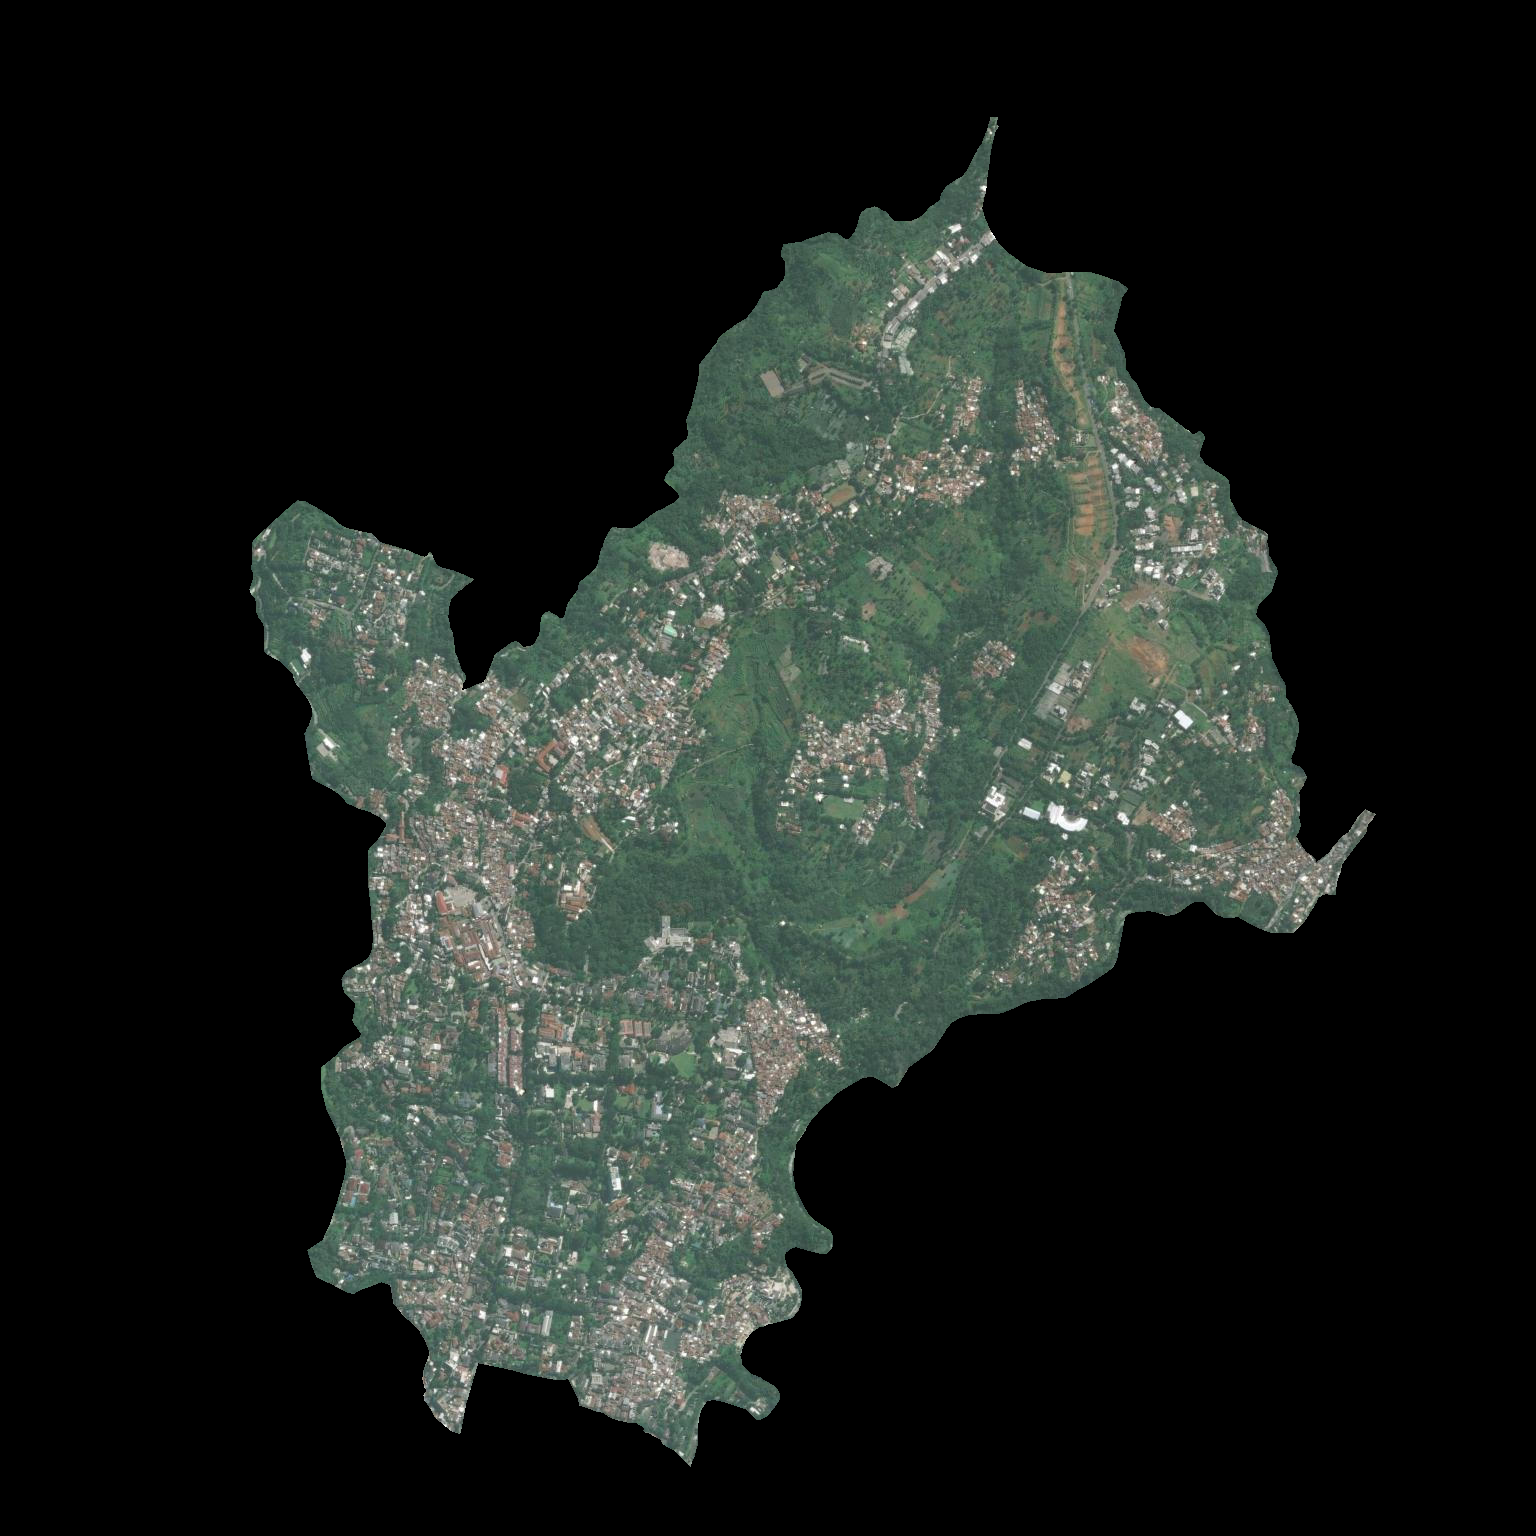
\includegraphics[width=0.6\textwidth]{Gambar/Ciumbuleuit.png}
	\caption{Kelurahan Ciumbuleuit}
	\label{fig:ciumbuleuit}
\end{figure}

Dari hasil penelitian Juan A. Kusjadi yang menghasilkan data  berupa gambar terlihat seperti pada gambar \ref{fig:ciumbuleuit}, merupakan hasil proses gambar sebuah kelurahan Ciumbuleuit. Proses pengekstraksian gambar tersebut dilakukan dengan mengakses ke tempat penyimpanan data \textit{Hadoop Distributed File System}(HDFS)\footnote{File system terdistribusi yang beroperasi di \textit{hardware} standar maupun \textit{low-end}.}. Untuk mendapatkan akses ke sistem \textit{hadoop} harus menggunakan akun yang diterdaftar pada laboratorium Fakultas Teknologi Sains dan Informatika (FTIS) di Universitas Katholik Parahyangan (Unpar). Setelah dapat mengakses akun tersebut barulah dapat mengunduh data. Data yang dapat diambil masih dalam format ".txt" dengan nama Kota\_Bandung, dalam pengambilan data Kota\_Bandung.txt menggunakan perintah yang telah tersedia pada HDFS. Data Kota\_Bandung.txt masih tersimpan pada di dalam server dan dengan menggunakan \textit{command-line interface} untuk mengunduh data tersebut ke \textit{local directory}.

Data Kota\_Bandung.txt yang berhasil diunduh masih memiliki format file ".txt" di mana setiap baris menyatakan sebuah \textit{tile} dari gambar kelurahan atau kecamatan. Setiap \textit{tile} harus terlebih dahulu di-\textit{decode} dari base 64\footnote{Algoritma Base64 merupakan salah satu algoritma untuk \textit{Encoding} dan \textit{Decoding}.} menjadi gambar yang memiliki format ".png". Proses mendapatkan gambar kelurahan atau kecamatan Kota Bandung secara utuh, harus dilakukan penggabungan setiap \textit{tile} dari gambar kelurahan atau kecamatan.

Proses pengekstraksian \textit{tile} dilakukan dengan menggunakan bahasa pemrograman Python\footnote{Python adalah bahasa pemrograman yang banyak digunakan dalam aplikasi web, pengembangan perangkat lunak, ilmu data, dan \textit{machine learning} (ML). Developer menggunakan Python karena efisien dan mudah dipelajari serta dapat dijalankan di berbagai platform.}. Berbagai macam \textit{library} yang dapat digunakan pada bahasa pemrograman Python dalam membantu pengembangan laman web, diantaranya menggunakan \textit{Python PIL(Pillow)} yang berguna untuk menggabungkan gambar, dan \textit{library} base 64 yang digunakan dalam melakukan peng-\textit{decode}-an teks yang merupakan sebuah \textit{tile} gambar kelurahan atau kecamatan.

Pengembangan halaman website dapat dilakukan dengan menggunakan data-data yang telah terkumpul. Data yang terkumpul termasuk didalamnya luas wilayah, luas area hijau, dan kebutuhan area hijau di setiap kelurahan atau kecamatan. Dalam pengembangan halaman website juga terdapat data gambar berupa gambar citra satelit dan gambar luas area hijau kelurahan atau kecamatan. Dengan dikembangkan halaman website pemvisualisasi ruang terbuka hijau di Kota Bandung maka pengguna dapat memenuhi kebutuhan tempat tinggal bagi masyarakat agar dapat beraktivitas dengan normal dan mendapatkan kadar oksigen yang merata. 


\section{Rumusan Masalah}
\label{sec:rumusan}
Berdasarkan deskripsi dan latar belakang yang sudah dibahas bahwa rumusan masalah yang muncul adalah sebagai berikut:

\begin{itemize}
	\item Bagaimana membuat sebuah halaman website interaktif yang dapat membandingkan data dua buah kelurahan atau kecamatan Kota Bandung?
	\item Bagaimana cara pengguna untuk membandingkan atribut-atribut Citra Satelit dari kelurahan atau kecamatan Kota Bandung?
	\item Bagaimana cara mengekstraksi data citra satelit pada HDFS ke \textit{local directory}?	
\end{itemize}

\section{Tujuan}
\label{sec:tujuan}
Tujuan dari skripsi ini adalah:
\begin{enumerate}
	\item Membuat sebuah halaman website interaktif yang dapat membandingkan dua lokasi kelurahan.
	\item Pengguna dapat memilih kecamatan atau kelurahan untuk sisi kiri dan kanan, untuk membandingkan atributnya.
	\item Data citra satelit yang didapatkan akan digunakan untuk memenuhi kebutuhan pada lawan web yang akan dibangun.
\end{enumerate}


\section{Batasan Masalah}
\label{sec:batasan}

Batasan-batasan masalah untuk penelitian ini adalah sebagai berikut:
\begin{enumerate}
	\item Penelitian dari data yang sudah matang.
\end{enumerate}

\section{Metodologi}
\label{sec:metlit}
Metodologi yang akan digunakan dalam pembuatan skripsi adalah:
\begin{enumerate}
	\item Melakukan survei kepada Fritz H. Hutapea SKom dan Juan A. Kusjadi terkait penenilitiannya
	\item Melakukan pengumpulan data hasil penelitian
	\item Mempelajari ekstraksi data citra satelit yang disimpan pada HDFS
	\item Mempelajari bahasa pemrograman php, html, css dan cara menggunakan \emph{framework} laravel.
	\item Mempelajari kebutuhan laman web.
	\item Melakukan analisis kebutuhan laman web.
	\item Melakukan perancangan antar muka laman web.
	\item Membangun laman web bedasarkan \emph{framework} Laravel.
	\item Melakukan pengujian pada laman web.
	\item Menulis dokumen skripsi.
\end{enumerate}

\section{Sistematika Pembahasan}
\label{sec:sispem}
%Rencananya Bab 2 akan berisi petunjuk penggunaan template dan dasar-dasar \LaTeX.
%Mungkin bab 3,4,5 dapt diisi oleh ketiga jurusan, misalnya peraturan dasar skripsi atau pedoman penulisan, tentu jika berkenan.
%Bab 6 akan diisi dengan kesimpulan, bahwa membuat template ini ternyata sungguh menghabiskan banyak waktu.

Skripsi ini disusun dalam beberapa bab secara sistematis sebagai berikut:
\begin{itemize}
	\item \textbf{Bab 1 Pendahuluan} \\ 
	Berisikan tentang latar belakang, rumusan masalah, tujuan, batasan masalah, metodologi, dan sistematika pembahasan.
	\item \textbf{Bab 2 Landasan Teori} \\ 
	Berisikan tentang dasar-dasar dari teori-teori yang digunakan dalam membangun halaman web seperti \textit{Command-line interface}, \textit{Hadoop Distributed File System}, \textit{Python} beserta \textit{library}-nya, Base 64, dan \textit{Framework}.
	\item \textbf{Bab 3 Analisis} \\ 
	Pada bab ini akan menjelaskan proses pembentukan gambar didalamannya terdapat bagaimana cara pengunduhan teks, pengkonversian baris menjadi gambar, dan menggabungkan gambar. Juga terdapat analisis kebutuhan perangkat lunak.
	
\end{itemize}
